\documentclass[a4paper]{article}

\usepackage{amssymb,mathrsfs,amsmath,amscd,amsthm}
\usepackage[mathcal]{euscript}
\usepackage{stmaryrd}
\usepackage[T1]{fontenc}
\usepackage{enumitem}
\usepackage{titling}
\usepackage{float}

%Image-related packages
\usepackage{graphicx}
\usepackage{subcaption}
\usepackage[utf8]{inputenc}
\usepackage[export]{adjustbox}
\graphicspath{ {../plots/} }
%------------------------------

\setlength\parindent{0pt}

\title{Report}
\author{Marcin Mazur}

\begin{document}

\maketitle

\section{Architecture}
For the \textit{Coupling Layers} I used simple MLPs with \textit{LeakyReLU} and
\textit{BatchNorm1d}. I tried many activation functions: \textit{ReLU}, \textit{Sigmoid},
\textit{Tanh}, but \textit{LeakyReLU} turned out to give the best results. When it
comes to batch norm I tried to minimize momentum as much as possible (as far as training
did not become unstable). In \textit{RealNVP} I decided to go for 10 Coupling Layers of
5 flavours (different sizes of MLPs). Each flavour first was applied to first half of input
vector and then second half (simply use the same configuration twice, one after another).

\section{Optimization}
For the optimization I used \textit{Adam} with warm-up and reducing on plateau.
Model tended to learn best till approximately $60$ epoch, after that progress was very slow.
\newpage

\section{Results}
I reached minimal $-1600$ loss, but could not get better scores. I think that was
caused by the fact that model was not complex enough (more complex models
gave me 'CUDA out of memory' errors, so I sticked to the final model presented
in notebook).

\begin{figure}[H]
    \centering
    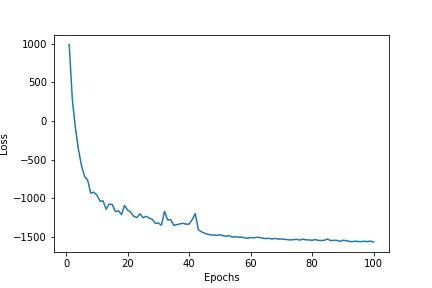
\includegraphics[height=8cm]{Loss_04-Jun-2022-18.png}
    \caption{Loss}
\end{figure}

As you can see fives produced by sampling from normal distribution and passed to model
inverse flow are pretty good. The samples produced by model definitely look very alike
and tend to be better (when it comes to symmetry, precision, etc.) than handwritten digits.

\begin{figure}[H]
    \centerline{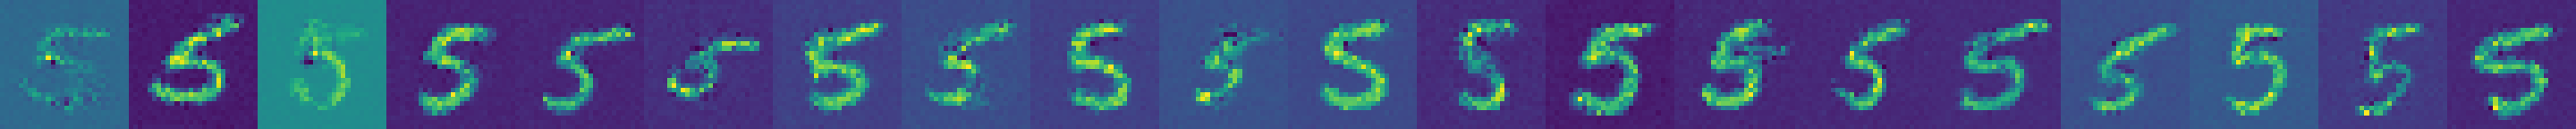
\includegraphics[width=1.1\textwidth, height = 1.5cm]{Samples_05-Jun-2022-20.png}}
    \caption{Samples}
\end{figure}

\end{document}
